% This is the Reed College LaTeX thesis template. Most of the work 
% for the document class was done by Sam Noble (SN), as well as this
% template. Later comments etc. by Ben Salzberg (BTS). Additional
% restructuring and APA support by Jess Youngberg (JY).
% Your comments and suggestions are more than welcome; please email
% them to cus@reed.edu
%
% See http://web.reed.edu/cis/help/latex.html for help. There are a 
% great bunch of help pages there, with notes on
% getting started, bibtex, etc. Go there and read it if you're not
% already familiar with LaTeX.
%
% Any line that starts with a percent symbol is a comment. 
% They won't show up in the document, and are useful for notes 
% to yourself and explaining commands. 
% Commenting also removes a line from the document; 
% very handy for troubleshooting problems. -BTS

% As far as I know, this follows the requirements laid out in 
% the 2002-2003 Senior Handbook. Ask a librarian to check the 
% document before binding. -SN

%%
%% Preamble
%%
% \documentclass{<something>} must begin each LaTeX document
\documentclass[12pt,twoside]{reedthesis}
% Packages are extensions to the basic LaTeX functions. Whatever you
% want to typeset, there is probably a package out there for it.
% Chemistry (chemtex), screenplays, you name it.
% Check out CTAN to see: http://www.ctan.org/
%%
\usepackage{graphicx,latexsym} 
\usepackage{amssymb,amsthm,amsmath}
\usepackage{longtable,booktabs,setspace} 
\usepackage{chemarr} %% Useful for one reaction arrow, useless if you're not a chem major
\usepackage[hyphens]{url}
\usepackage{rotating}
\usepackage{natbib}
\usepackage{listings}
\usepackage{color}

\definecolor{dkgreen}{rgb}{0,0.6,0}
\definecolor{gray}{rgb}{0.5,0.5,0.5}
\definecolor{mauve}{rgb}{0.58,0,0.82}

\lstset{frame=tb,
  language=Java,
  aboveskip=3mm,
  belowskip=3mm,
  showstringspaces=false,
  columns=flexible,
  basicstyle={\small\ttfamily},
  numbers=none,
  numberstyle=\tiny\color{gray},
  keywordstyle=\color{blue},
  commentstyle=\color{dkgreen},
  stringstyle=\color{mauve},
  breaklines=true,
  breakatwhitespace=true,
  tabsize=3
}
% Comment out the natbib line above and uncomment the following two lines to use the new 
% biblatex-chicago style, for Chicago A. Also make some changes at the end where the 
% bibliography is included. 
%\usepackage{biblatex-chicago}
%\bibliography{thesis}

% \usepackage{times} % other fonts are available like times, bookman, charter, palatino

\title{PowerPoint Natively on the Web, a JavaPPTX Extension}
\author{Dylan H. Huff}
% The month and year that you submit your FINAL draft TO THE LIBRARY (May or December)
\date{May 2019}
\division{Mathematics and Natural Sciences}
\advisor{Eric S. Roberts}
%If you have two advisors for some reason, you can use the following
%\altadvisor{Your Other Advisor}
%%% Remember to use the correct department!
\department{Computer Science}
% if you're writing a thesis in an interdisciplinary major,
% uncomment the line below and change the text as appropriate.
% check the Senior Handbook if unsure.
%\thedivisionof{The Established Interdisciplinary Committee for}
% if you want the approval page to say "Approved for the Committee",
% uncomment the next line
%\approvedforthe{Committee}

\setlength{\parskip}{0pt}
%% End Preamble
%%
%% The fun begins:
\begin{document}

  \maketitle
  \frontmatter % this stuff will be roman-numbered
  \pagestyle{empty} % this removes page numbers from the frontmatter

% Acknowledgements (Acceptable American spelling) are optional
% So are Acknowledgments (proper English spelling)
    \chapter*{Acknowledgements}
	I want to thank a few people.

% The preface is optional
% To remove it, comment it out or delete it.
%   \chapter*{Preface}
%	This is an example of a thesis setup to use the reed thesis document class.
	
	

    \chapter*{List of Abbreviations}
	\begin{table}[h]
	\centering % You could remove this to move table to the left
	\begin{tabular}{ll}
		\textbf{API} & Application Programming Interface\\ 
		\textbf{CS}   & Computer Science\\
		\textbf{HTML} & Hyper Text Markup Language\\
		\textbf{JS}  	&  JavaScript\\
	\end{tabular}
	\end{table}
	

    \tableofcontents
% if you want a list of tables, optional
%   \listoftables
% if you want a list of figures, also optional
    \listoffigures

% The abstract is not required if you're writing a creative thesis (but aren't they all?)
% If your abstract is longer than a page, there may be a formatting issue.
    \chapter*{Abstract}
	Computer Science higher education is facing a growing crisis, there aren't enough faculty members to support student demand. This problem shows no sign of getting any better in the years to come as the amount of people getting Ph.D.s annually who intend on working as a professor is far fewer than the number of unfilled faculty positions. Various tools have been created for Computer Science professors that free up time so that they can focus on students. There are tools for automating grading, animation creation and presentation creation. This thesis focuses on one package, JavaPPTX. This package allows people to make complicated PowerPoint animations in Java. Having a package that can do this is important because teaching topics such as recursion, stacks, sorting algorithms and others can be graphically demanding. Making these presentations in Java allows the user to have precision that would be very difficult to get using Microsoft PowerPoint. My contribution to this package is the addition of compilation of the Java code to JavaScript and HTML. With only adding two additional lines of code on the users part, a web native version of the presentation will also be made. This allows presenters to make websites that are identical to their presentations with marginal additional effort. From the students perspective, this gives them the option to view the presentation on any internet connected device without needing any additional software. In an age where cellphones are increasingly the way people access the internet, my extension adds convenience for some, while allowing the presentation to be viewed by audiences who wouldn't otherwise be able to access it. 
	
	\chapter*{Dedication}
	I'd like to dedicate this to my parents, who have sacrificed so much over their entire lives to allow me to get this education. I love you both and will always be grateful for this gift. 

  \mainmatter % here the regular arabic numbering starts
  \pagestyle{fancyplain} % turns page numbering back on

%The \introduction command is provided as a convenience.
%if you want special chapter formatting, you'll probably want to avoid using it altogether

    \chapter*{Introduction}
         \addcontentsline{toc}{chapter}{Introduction}
	\chaptermark{Introduction}
	\markboth{Introduction}{Introduction}
	In order to support the already strained Computer Science professors, I created an extension to the JavaPPTX package that allows presentations to be web native. This presentations would be programmed in Java, but the output is JavaScript and HTML. My extension to package can be accessed at \begin{quote} https://github.com/dylanhuff/thesis-code \end{quote} The most up-to-date version of JavaPPTX and any further expansion or extensions can be accessed at \begin{quote} https://github.com/eric-roberts/JavaPPTX \end{quote} The rest of this thesis will be broken down as follows. Chapter 1, I give define algorithm animation and explain its usage in Computer Science education. In Chapter 2, I describe the state of computer science higher education in 2019 and where it is forecast to go in the coming years. This chapter also includes some proposed solutions to combat the current faculty shortage. In Chapter 3 I explain the functionality I added to JavaPPTX and how it works. This chapter also includes some of the technical challenges I faced along with way and how my extension could be expanded. 
	
\chapter{Algorithm Animation}
	
\section{What is Algorithm Animation and Why is it Important?}	
Algorithm animation is the process of taking algorithms and giving them graphical representations. Algorithm animation has benefits for teachers and students. Below are some of the most commonly cited benefits.\footnote{\cite{hundhausen_meta-study_2002}}
\begin{itemize}
\item It allows teachers to display algorithms in lectures easily.
\item Another method for teaching students fundamental algorithms, it adds a more visual element rather than just showing code. 
\item It allows for another avenue of debugging. 
\end{itemize}
\begin{figure}[htbp] 
\begin{centering} 
\caption{Example of an Algorithm Animation \footnotesize{Source: https://visualgo.net/en/bst}}
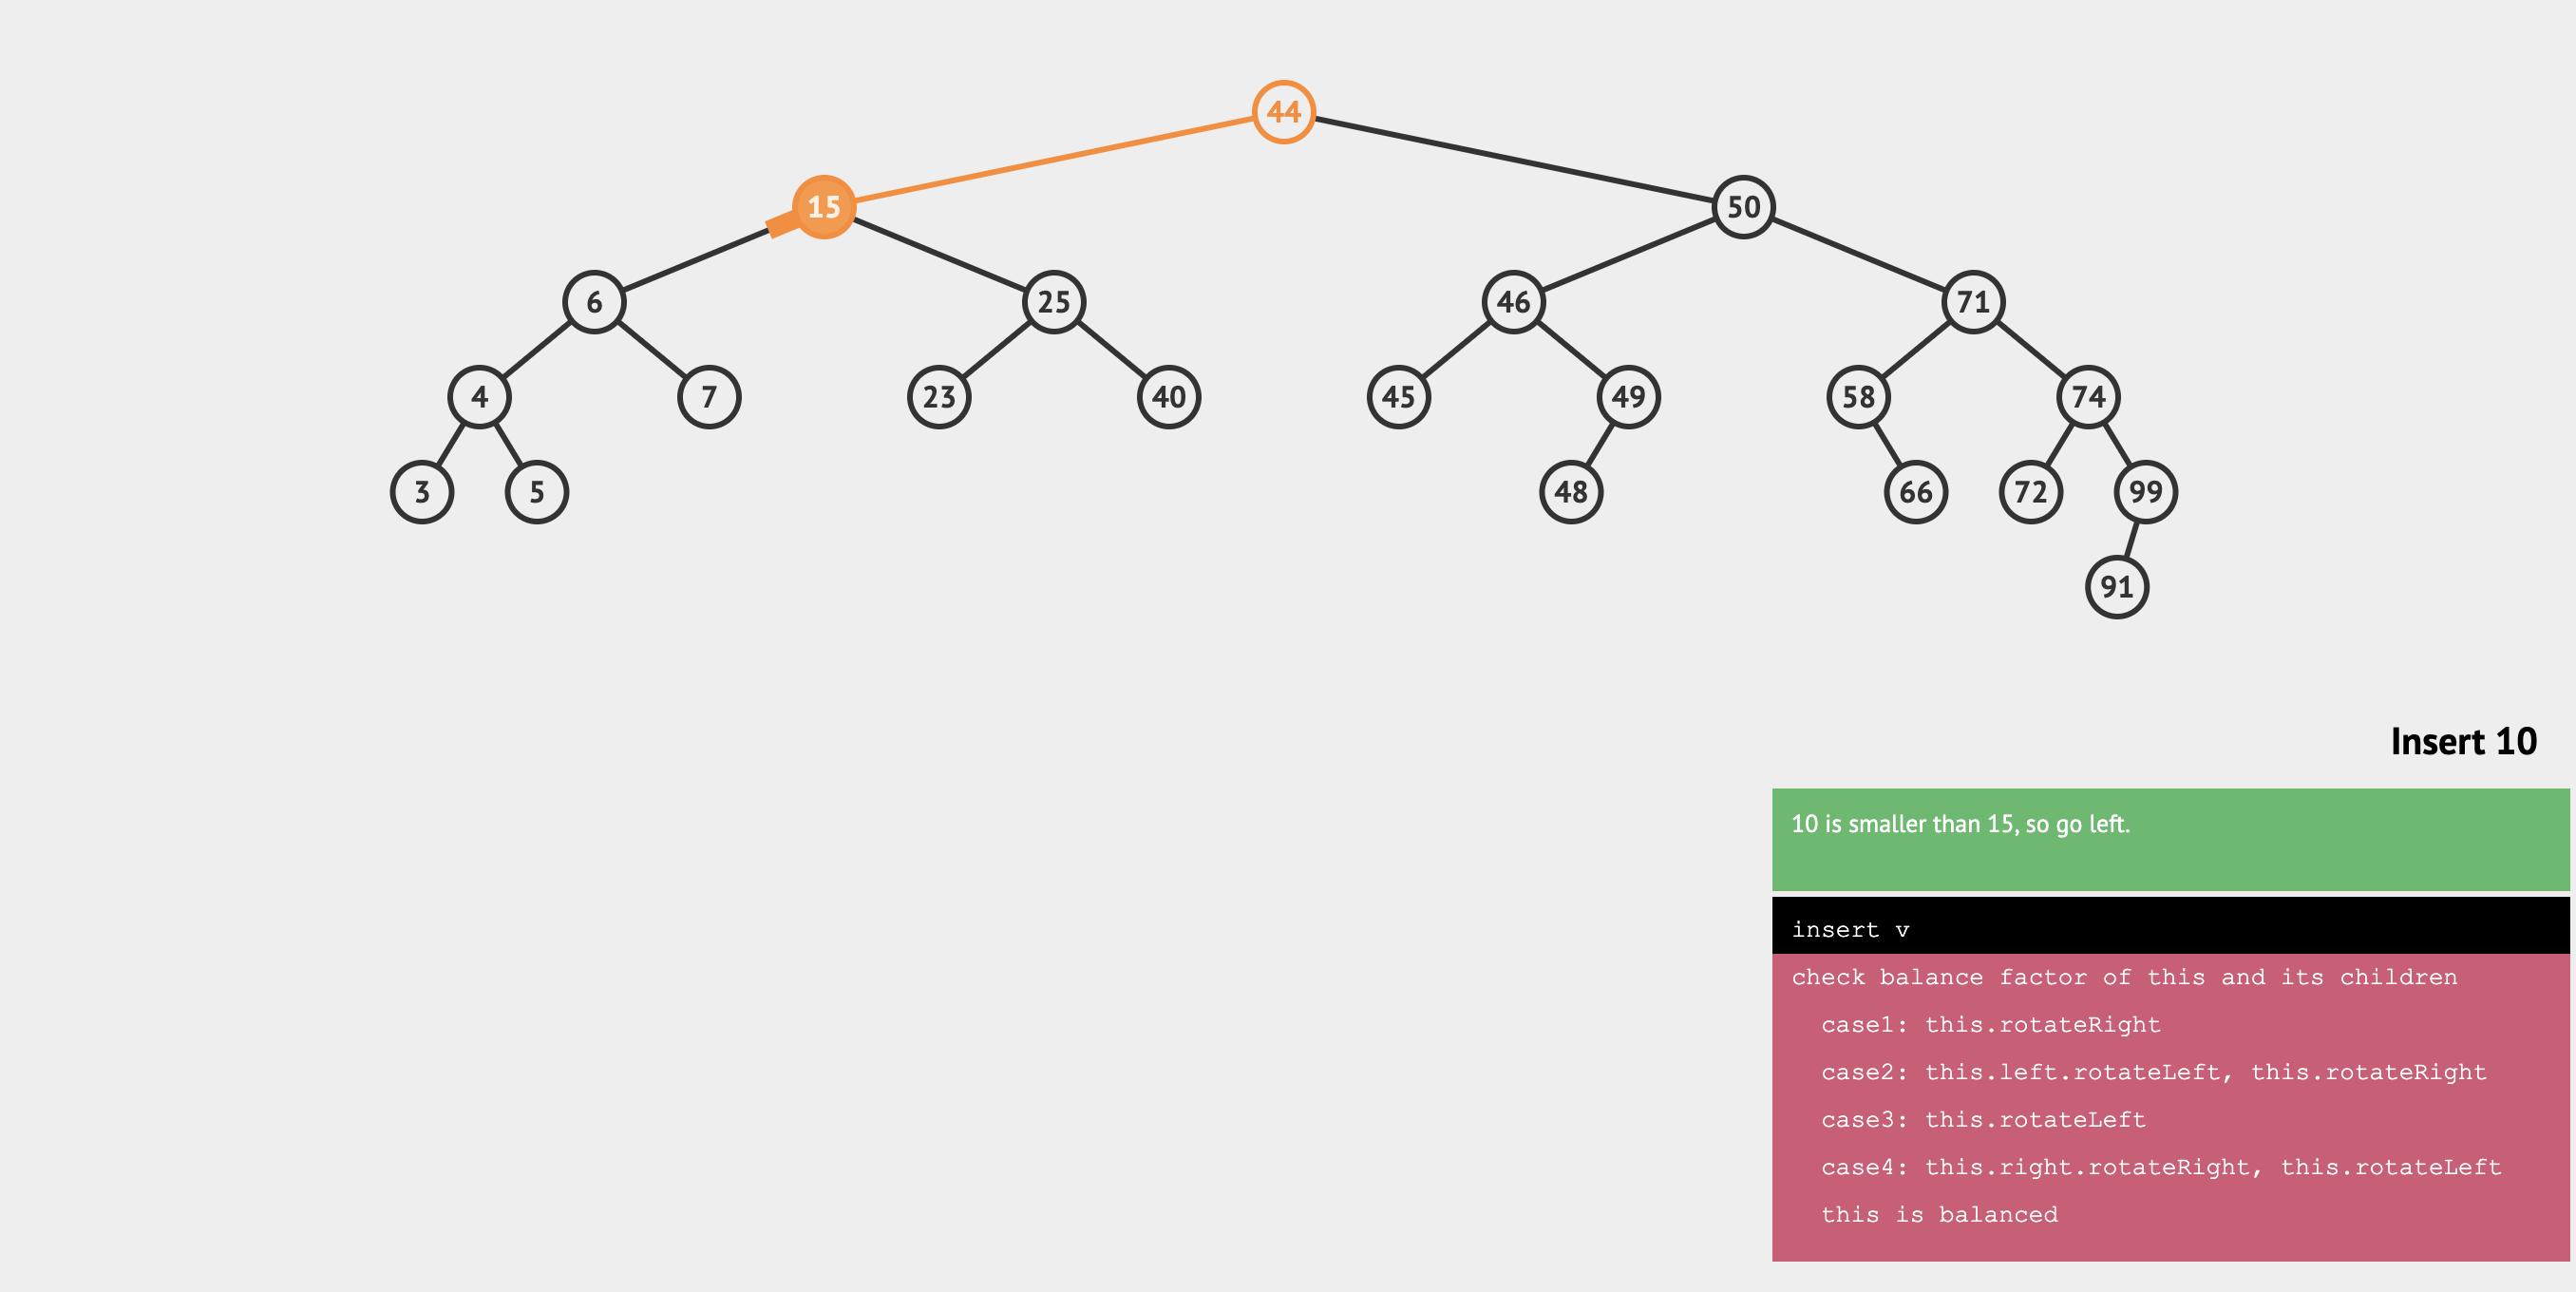
\includegraphics[scale=0.32] {animexample}
\label{animexample}
\end{centering} 
\end{figure}


\section{Use in Computer Science Education}

\subsection{History}
Algorithm animation began in the 70's and has seen usage since. In the early days of algorithm animation, teachers used tools to make animations for their presentations. Often time these were predefined short films. As tools progressed, the animations no longer had to be used exclusively by teachers and didn't need to be predefined.\footnote{\cite{hundhausen_meta-study_2002}} Tools became able to dynamically represent the algorithms that students made. 

One of the most famous and important contributions to algorithm animation was BALSA. BALSA was created in 1987 by Marc Brown. BALSA introduced several major innovations in the field. One major contribution was the addition of real time animations. Prior to BALSA, the animations wouldn't operate in real time, rather the animation would algorithm would run then the animation would be made, unlike real time animation which executes the animation and algorithm simultaneously. Another innovation was the introduction of scripts. Scripts were predefined PASCAL programs that would control the algorithm and could be executed in real time. This allows teachers to predefine how an animation will execute, then present the animation in real time.\footnote{\cite{brown_algorithm_1987}}

Along with this shift form predefined to dynamically defined tools, other features were added that improved the animations. One paritcularly notable improvment came in when animations transitioned from 2D to 3D. This shift from 2D to 3D allowed for more information to be simultaneously displayed. Along with this improvement, color and sound were both added to animations.\footnote{\cite{najork_library_1994}}

\subsection{Current State of Algorithm Animation}
There are a few challenges facing modern day algorithm animation. One of these challenges is the lack of adoption of animation tools by instructors.Levy points out two main challenges of adoption from survey results of teachers. The first is that the tools being developed may be feature rich but not integrated well into the existing material or curriculum. This illuminates the fact that the tool developers aren't usually primarily concerned with integration, but rather features. Second, they cite "centrality" as the other major inhibition of teachers. They define centrality to be 	where the center of learning is for the students. By making animation tools that animate the students algorithms, the centrality is being moved from the teacher to the student. They note that this phenomenon is present with highly confident and experienced teachers through not confidant inexperienced teachers.\footnote{\cite{levy_we_2007}}  Its also worth noting that the teachers in this study are high school teachers and not college professors. 

Along with low adoption rates by teachers, there is also a lack of work being published.\footnote{\cite{kucera_visualization_2018}}  


\chapter{State of Computer Science Higher Education}	
This chapter will be about the state of CS higher ed, its problems, some solutions and how JavaPPTX fits into that picture

\section{Background}
Talk about the history and formation. Talk about its periods of growth and bust. Talk about current growth and future growth.

\section{Problems facing Higher Education}
Talk about various problems, how they arose and what their effects on education are.

\subsection{Lack of PhDs}
One of the major issues facing CS higher education is the amount of PhDs being produced and the percentage of them going to industry versus professor positions. Currently, 57\%of the new PhD graduates go to industry.\footnote{\cite{zweben_another_2018}} With wages in industry being considerably higher than wages for CS professors, there is no sign of this trend decreasing. 

Currently about 30\% of PhD graduates go into academia, but that doesn't mean they all take tenure track positions. About 10\% of all graduates choose to go into Post Doctoral positions while another 2\% go into research positions.\footnote{\cite{zweben_another_2018}} In the end, only 18\% end up in teach positions. This translates to 320 graduates. To put that in perspective, there are currently 1577 open faculty positions in 2015. While those numbers seem bleak, the picture only gets worse. Consider that when large prestigious universities have openings, the graduates are much more likely to go there compared to smaller local universities with less prestige. 

\subsection{Increasing Demand from Students}
Between 2009 and 2015, the amount of people graduating with a bachelors degree from not-for-profit institutions has increased 74\%. This is significantly higher than the general rate of increase in bachelors degrees awarded over the same period of time. This is the average increase. As the books notes, their is large variation between institutions, with some seeing rates much higher than the average. In particular, research institutions tend to see higher than average rates of increase. Another consideration with this average is that some institutions also work to cap the amount of prospective CS students they admit. It is worth noting that there have been major increases in the past, followed by sharp decreases. There is no one factor that can account for the historical decreases in the past.  \footnote{\cite{committee_on_the_growth_of_computer_science_undergraduate_enrollments_assessing_2018}} 

On top of increased degree production, enrollment of CS courses from CS majors and non-majors has also increased since 2005. This trend also shows no sign of slowing down within the next few years, relative to 2018, without any institutional discouragement. 

One of the major reasons for this increased demand is that in the U.S.,  the number of jobs related to computing have been increasing steadily for the past 40 years. Currently, there are not enough students graduating with degrees relating to the field to fill open the current open job positions. Looking down the road, the U.S. Bureau of Labor Statistics estimates that the number of jobs in this area is estimated to continue to grow rapidly through atleast 2026.\footnote{\cite{BLS}} Beyond the data predicting continued growth, given the increasing pervasiveness of computers in the world, it makes sense that the amount of jobs will continue to grow for the foreseeable future. 

\section{Proposed Solutions}

Currently there is no definitive solution to the problems facing CS Higher Education. Most of the problems stem from the job market and there is no sign that the job market will ease up on the pressure that it is applying. There are a few solutions that have been proposed, none of which will be the sole answer.

Stanford recently implemented a program to retrain Ph.D.s from others disciplines.\footnote{\cite{starkman_stanford_0400}} The program is a Masters of Education which will teach these people fundamental CS skills. The goal of this program is not to have these people teaching advanced CS courses, but rather have them be the teachers for some of the introductory courses. These retrained faculty also do not need to participate in outside research, rather their main focus would be teaching courses. This solution should help free up the faculty that has more advanced knowledge, allowing them to teach the high level courses and do their research. As an added benefit, it maybe the case that since the people being retrained are committed academics, they could be less likely to leave for industry. 

Another partial solution is the creation of supporting tools for existing faculty. In the next couple of years, there will not be enough professors to meet student demands. Even if a solution is found to get more professors, there will be years of delays before that solution is felt since it takes years to train people. Its obvious that more tools cannot replace faculty, but in terms of immediacy, tools have the advantage. There are existing auto grading tools for programming assignments which have been helpful. Another aspect of teaching that could be added is presenting. Tools could aid in the time it takes to create a presentation and the effectiveness that said presentation has. One tool in particular, JavaPPTX, will be the focus of this thesis.


\section{JavaPPTX}
JavaPPTx, created by Eric Roberts, is a library for Java that aids in the creation of PowerPoint Presentations. The package allows someone to write a program in Java that will create a PPTX file. This differs from the usual method of creating PowerPoints using Microsoft PowerPoint, which can become very cumbersome when making detailed animations that have specific movements or require many moving objects. 

\subsection{Background}
The package supports many of the features in PowerPoint and adds functionality in other cases. Here are some of the features supported:
\begin{itemize}
\item Creation of many shapes, including rectangles, ovals, lines, and more. 
\item Creation of text objects, including titles and long form text. 
\item Animation of objects. This includes fades, appearing, disappearing, linear motion, and more. All of these can be event based (clicks or delays). 
\item Support for multiple slides and slide transitions.
\item Importing of images.
\end{itemize}
Some of the extended functionality includes:
\begin{itemize}
\item An animated terminal function.
\item Exact animations including bezier paths. 
\item An animated stack tracing function.
\end{itemize}

\subsection{Classroom Usage}
One of the major benefits of the package is that it unobtrusively saves professors time while allowing them to animate hard to understand concepts.  The package fits in well because it doesn't require professors to change their teaching methods, as many professors already use PowerPoint during their lectures. While their is a learning curve associated with the package, it isn't particularly difficult to use and would save time in the long run. The package can be used to make simple slides, but the package was designed to, and excels at, making complicated PowerPoints. Some topics that can be more easily explained are recursion, loops, and debugging. 
\begin{figure}[htbp] 
\begin{centering} 
\caption{Example of an Algorithm Animation in JavaPPTX} 
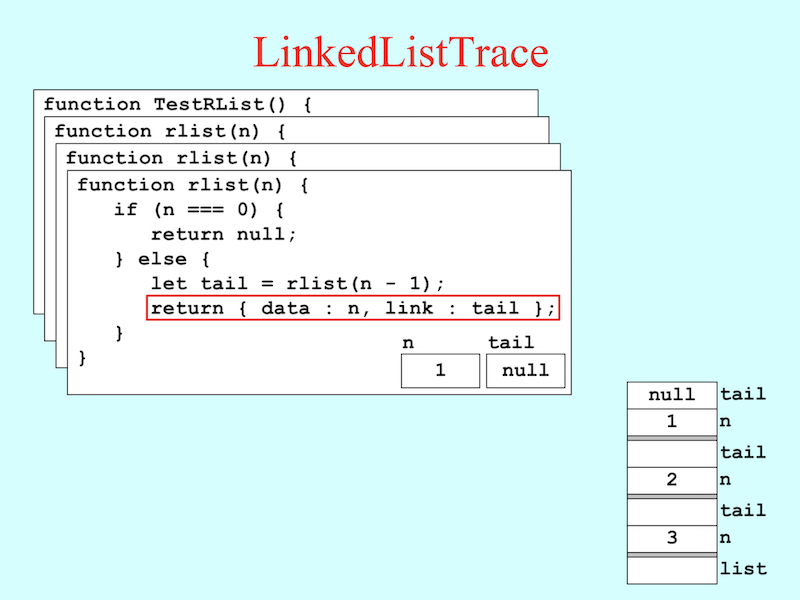
\includegraphics{algoanim} 
\label{subd}
\end{centering} 
\end{figure}
	
\subsection{Package Expansion}
Here I'll talk about ways that the package could be expanded and the benefits of the specific expansions. One will be my expansion. 

\chapter{JavaPPTX to JavaScript}

\section{Statement of Work}

\subsection{New Features}
The main addition of this work is he ability to export the presentation to HTML and JS without having to add any additional logic. This means that a professor could use JavaPPTX to create a PowerPoint for lecture, and with only having to add two lines the lecturer could create a web page that is identical to the PowerPoint. The newly created HTML file and JS file could be uploaded as is to create a web page, or could easily be embedded within an existing web page. 

Take the code in Figure 3.1 an example, which makes the previously shown Linked List Animation.
\begin{figure}[h!tbp]
\caption{Java Code for Linked List Animation} 
\begin{lstlisting}
import edu.stanford.cs.pptx.*;

public class PPLinkedListTrace {

   public void run() {
      PPShow ppt = new PPShow();
      PPCodeTraceSlide slide = new HSSlide();
      ppt.add(slide);
      ppt.save("LinkedListTrace.pptx");
      PPSaveJS testSave = new PPSaveJS(ppt);
      testSave.save("../example.js");
      System.out.println("LinkedListTrace.pptx");
   }

   public static void main(String[] args) {
      new PPLinkedListTrace().run();
   }
	...
}
\end{lstlisting}
\end{figure}
The only two lines that need to be added to export to JS and HTML are the lines shown in Figure 3.2.
\begin{figure}[h!tbp]
\caption{Two Lines for JavaScript Compilation} 
\begin{lstlisting}
		...
		testSave = new PPSaveJS(ppt);
		testSave.save("../example.js");
		...
\end{lstlisting}
\end{figure}
Another major addition was the automatic scaling to screen resolution. When a PowerPoint is created with this package, the slides will be a fixed size, defined in pixels. A major benefit of using JavaScript is the ability to scale the presentation without any additional work. This is an important feature because one benefit of outputting to web is that phones can natively view the presentation. With auto-scaling built in, the presentation will adjust to phones and desktops. 

\subsection{Uses of this Expansion}
Having a native web output has two main benefits, the ease of viewing the animation and allowing new audiences to view the animation. PowerPoint is not web native, meaning that someone that wants to view the lecture needs to download a copy of the PowerPoint and have access to an application that can view the PPTX file. While this isn't too large of a burden on laptops or desktops, accessing the lecture on a phone is very cumbersome and often infeasible. This barrier is easily overcome with HTML and JS as an output as almost all phones, as well as laptops and desktops, can view a web page easily. This is very convenient for anyone trying to view the lecture, but it also allows people without access to a laptop or desktop to view the lecture. 

\section{Internal Logic}
The process of building this feature set and making individual algorithms can be broken down into two parts, building the framework and cross compilation of the logic to the JavaScript framework.

\subsection{JavaScript Framework}
The JS framework relies heavily on the Canvas API. This API is meant to make animating in JS and HTML much simpler. The framework that I built is built on top of that and offers more abstractions to the programmer while also storing objects to be animated in a hierarchical and object oriented manner. This makes animating shapes and text objects much simpler. As an example consider drawing 5 circles and having them move using Canvas vs this framework. Canvas doesn't provide any way to keep track of drawn objects. It doesn't provide a native way to make objects move. It doesn't provide native re-rendering of drawn objects which is a problem when trying to move an object since it forces a rerender. Using the framework, a programmer would only need to create the 5 circle objects by passing them a few starting attributes (position, color, etc) then call a move function on the desired circle.

This framework creates classes for many of the shapes supported by JavaPPTX. The way that the framework was built allows for shapes classes to be easily added. The framework was created in a hierarchical manner, putting many of the methods into the abstract classes. This way, any objects added will have many of the methods already created for it. 

The framework is created dynamically, only building the parts that are necessary for that particular algorithm. This allows the resulting JS to be as minimal and fast as possible. This is done at compilation every time. There is some boilerplate framework that is created every time. 

\subsection{Cross Compilation}
After the framework is built, the logic is processed. The native JavaPPTX package stores all of the information passed by the programmer then creates the corresponding PowerPoint. Since all of the information is stored by the package prior to being complied to a pptx file, the information can be stored in the same way but compiled to JS. After a save to JS function is called, the program will crawl through all of the stored data, and run the corresponding compilation to JS functions. This step was particularly tricky because the way that Java stores information is different from JS, so all the logic needed to be translated. Take storing color data as an example. Java may store the color as "RED" but JS would take a hex string as a color attribute. This logic translation was possibly the most difficult part of creating this extension. It required understanding how Java and  JavaPPTX stored information, then figuring out the best way to store that in JS. Futhermore, the information can be stored in Java in a variety of ways. 

Translating from Java to JS was one set of problems, but another set of problems was translating between PowerPoints internal logic to JavaScripts. Most of the time, logic was stored in a manner that was clearly related to the object. For example, a rectangle would contain the length, width, color, position on the screen, etc. There were times that the information for an object was stored not based on what made sense for that object vacuously, but the information was stored with regards to the way PowerPoint needed to be given the information. One particularly troublesome example was lines. PowerPoint draws lines by keeping track of what quadrant of the slide the line is in. JS however doesn't render lines according to quadrant, so the logic needed to be translated before it is output. 

\section{Future Work}

\subsection{New Features}
What features did I miss? How can this overall be improved? This section will be quick to write once I know if/what features I was unable to get to. 

\subsection{Realtime JS Animation}
As this work stands, the animations that can be made are not real time and aren't reflecting algorithms that a student makes. A meta study has shown that it maybe more effective to have the animations reflect the students algorithms rather than having a teacher animate an algorithm and use it in a lecture, but this is contentious.\footnote{\cite{hundhausen_meta-study_2002}} A major contribution of this thesis is a JavaScript framework that allows for animations to be created more easily. In its current state, the animations are built based off of the logic given by the person creating the animation, which is intended to be an instructor. This framework could be used to reflect animations in real time that students create. Since the visual framework has been built, someone expanding on this work would have to figure out the logic behind creating animating the algorithms. The easiest expansion could be animating JS algorithms. Since JS is native to the web, it also maybe worthwhile to have other languages have animations done with this framework since the animations could easily be made into websites and shared. Since this package is written in Java, Java would be a logical language to expand this to. 


	
\chapter*{Conclusion}
         \addcontentsline{toc}{chapter}{Conclusion}
	\chaptermark{Conclusion}
	\markboth{Conclusion}{Conclusion}
	\setcounter{chapter}{4}
	\setcounter{section}{0}
	
Here's a conclusion
    \appendix
      \chapter{The First Appendix}


%This is where endnotes are supposed to go, if you have them.
%I have no idea how endnotes work with LaTeX.

  \backmatter % backmatter makes the index and bibliography appear properly in the t.o.c...

% if you're using bibtex, the next line forces every entry in the bibtex file to be included
% in your bibliography, regardless of whether or not you've cited it in the thesis.
    \nocite{*}

% Rename my bibliography to be called "Works Cited" and not "References" or ``Bibliography''
% \renewcommand{\bibname}{Works Cited}

%    \bibliographystyle{bsts/mla-good} % there are a variety of styles available; 
%  \bibliographystyle{plainnat}
% replace ``plainnat'' with the style of choice. You can refer to files in the bsts or APA 
% subfolder, e.g. 
 \bibliographystyle{APA/apa-good}  % or
 \bibliography{thesis}
 % Comment the above two lines and uncomment the next line to use biblatex-chicago.
 %\printbibliography[heading=bibintoc]

% Finally, an index would go here... but it is also optional.
\end{document}
